\chapter{System fundamentals}
Not all operating systems will be covered in this thesis.
The following statements are true for the testing machines used in chapter 4?.
\section{Processes}
To many operating systems a process is like an wrapper defined by the kernel in order to allocate resources to an executing program.\\
When a process is created the system assigns him a \textit{process unique identifier} also called PID(a positive integer). Each process has its own PID, so two different executing programs cannot have the same PID \footnote{On UNIX like machines the first process to be called is the init process with PID 1}. The methods used to create a new process differ on each operating systems.
On Windows you can create processes by calling the \texttt{CreateProcessA()} function \cite{createProcWinAPI}, which returns a HANDLE (the equivalent PID for windows systems) and on linux you can use \texttt{fork()}\cite{LPI}. Each operating system calls one these methods internally every time the computer or the user starts a routine of execution, like starting a service, or a program (browser, spotify, etc). You can think of this system like a binary tree with one or more children with the kernel on top. The children have also an additional attribute called PPID, that contains the PID of its creator. If this is specified to zero then the kernel is the parent.\cite{wikiPPID}\footnote{There a very few processes that have the PPID=0 (ex. init)}.
\subsection{Threads} 
Each process has at least one thread of execution called the main thread, which as the name say contains the \texttt{main()} function. Once a thread has been created, the main thread has to wait for it to finish by calling a method called \texttt{join()}. As their creators, threads also have unique identifiers called \textit{Thread identifiers} or TID and OS-specific methods to create them. On UNIX systems one would use the \texttt{pthread\_create()} and on windows \texttt{Create\_Thread()}. But the role of this library is to make this whole process as easy as possible, so we will use the C++ Standard Library's threads (std::thread) and \dq detach\dq{}\footnote{There is also a method called \texttt{detach()} which allows a thread to separates itself from the main thread. This way the thread can terminate itself and the main thread doesn't have to wait for that thread's termination} ourselves from the other ones.\\
Processes have their own stack, so they can't communicate with each other. This is a huge problem when it comes concurrency (explained in \autoref{ssec:c	oncurrency}), but threads share the stack of their creator-process.
\subsection{Differences between threads and processes} 
Many people tend to think of threads and processes as being the same, but they are quite different. First as mentioned above threads share the same stack of the creator-process, while processes need intercommunication tools like pipes to talk to each other. Another difference is that a process can have multiple threads attached to it, but a thread cannot belong to more than one process.\footnote{If the execution method of a thread calls \texttt{fork()} then that process's PPID will be the PID of thread's creator}. Their identifiers are also independent from their creator's. This way a TID can be equal to its creator's (or another process's) PID. \\
One can imagine a process like an octopus and the threads being it's arms. One octopus has many arms that can execute multiple tasks at the same time, but an arm cannot belong more than one octopus.\\
In this library we use multiple threads to simulate a user specific workload because this way we can time their execution start point with only one shared variable and we don't have to worry about interprocess communications. 
\subsection{Attributes}
Normally when we would create a threads using the unix methods, we would pass a pointer to a
structure that describes the attributes for that specific thread(that structure can be created with 
\texttt{pthread\_attr\_init()} and be destroyed with \texttt{pthread\_attr\_destroy()}. Some of these attributes include the 
scheduling priority, scheduling policy and stack size, which are important for out tests. 
Unfortunately the standard library doesn't have this option. In order to set and get this attributes
we need to use the architecture's dependent functions. 
\subsection{Stack Size}
\begin{wrapfigure}{1}{0.5\textwidth}
	\centering
	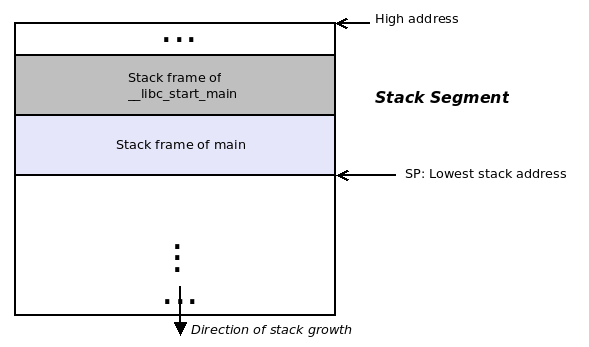
\includegraphics[width=.98\linewidth]{../figures/systemgrundlagen/stack.png}
	\caption{Stack segment}
	\cite{stack}
\end{wrapfigure}
The stack is a piece of memory where meta-data and local variables are saved when the \texttt{main()} function calls a routine/method. This memory segment is limited and doesn't allow an infinite number of data segments (also called stack frames) being stored in it. The stack uses assembly instruction like \texttt{pop} to delete a frame and \texttt{push} to add a frame. For consistency the stack will always pop the last element pushed. This is also known as \dq Last in First Out\dq{}\cite{stack}.\\
On UNIX systems we would create an attribute structure and pass the
desired options there. But because we don't use the unix's system function \texttt{pthread\_create()} we also
cannot use the attribute structure. Furthermore the standard library doesn't support such tweaks. 
This is very important if someone wants to use this for an ARM architecture, because he won't be
able to define a meaningful stack size. This doesn't pose any threats for many operating systems out
there, but for ARM, which has a limited stack size can be problematic. For windows this attribute
can be set using the \texttt{Create\_Thread()} function just like in unix using \texttt{pthread\_create()}.
\newpage
\section{Concurrency}
\label{ssec:concurrency}
Concurrency means that two or more things are happening simultaneously. This pehnomenon is happening
everyday almost everywhere we look. Even we as humans are capable of such thing, for example walking
and talking at the same time. In computer science concurrency means that more than one process can
be execuvted at the same time. Many systems have this ability, because most of them are
multiprocessor computers. Even some single core computers can handle concurrency to some extent.
One calculation unit can handle one task at a time, but it can quickly switch to another task if
necessary. This is why sometime even single core units give the impression of resolving jobs
simultaneously\cite{concurrency}. Although performant this method does not come without its flaws. When a cpu gets a new task, the resources of the old task (eg. local variable, meta data of the current task, etc.)will be replaced by those of the new job. This is also known as \dq Context Switching\dq{}.
The order of task switching will be explained in detail in chapter *scheduling*.\\ 
Nowadays many systems measure the concurrency of a system by its number of hardware threads. This
unit of measure tells us how many independet tasks can the processor handle.
\section{CPU Affinity}
The affinity of a CPU determines the number of processors that one process can use for its threads.
This library offers methods to restrict the number of CPUs off which a process can run on. This is
sometimes desirable because of the following reasons:
\begin{enumerate}
	\item Data invalidation: When a process starts, the user cannot tell from outside on which CPU
	that thread started. When a process finishes its time-slice, he has to give up its CPU for
	others to use it and it come back later, but it won't necessarily start on the same CPU as the
	last time. \footnote{This is a part of context switching, which was discussed in chapter \ref{ssec:concurrency}}. When this happens, entries in that CPU's cached must be replace or removed,
	which is known as \dq Cache invalidation\dq{}. This is not a flawless method and cache inconsistencies
	can appear.
	\item Emergency CPU: On real-time systems, where human lives are at risks, many developers will
	deliberately block some CPUs ( on a multicore machine) to use them when the system returns
	erros and needs to immediately execute safety protocols. Because the CPUs were blocked
	from being used on other processes, these remain free and so the execution of the safety procedure can start without any delay (eg. context switching).
	
\end{enumerate}

By default most systems allow each process to use all CPUs. If the user turns off half of the
CPUs of a given process and tries to create an additional workload with the library's methods for that process, he must keep in
mind that the workload will also be cut in half because the threads have less processors to work on.
\section{Priorities}
When it comes to the priority of a process there is a big difference between a UNIX system and a
windows machine. On windows the priority is determined by the priority class of the process and the
its thread priority.\\
\subsection{Windows}
Based on the winAPI documentation\cite{priorityClasses}, the classes can have the following values:
\begin{enumerate}
	\item IDLE\_PRIORITY\_CLASS (0x00000040): This is the lowest priority, processes belonging to this class run only if the system is idle and can be preempted\footnote{If a process is preempted that means it stops executing and yields the cpu} by a process with a higher priority
	\item BELOW\_NORMAL\_PRIORITY\_CLASS(0x00004000): This class has a higher priority than an idle-classed process but a lower priority than a normal-classed process 
	\item NORMAL\_PRIORITY\_CLASS(0x00000080
	): This is the default class for all processes created by the user
	\item ABOVE\_NORMAL\_PRIORITY\_CLASS(0x00008000): This class has a higher priority than an normal-classed process but a lower priority than a high-classed process
	\item HIGH\_PRIORITY\_CLASS(0x00000080): This class is usually used for time critical jobs
	\item REALTIME\_PRIORITY\_CLASS(0x00000100): This is the class with the highest priority and is rarely used because it stop most of the tasks on the calling machine
\end{enumerate}
Each class can be preempted by a higher priority class besides the realtime-class. Classes categorize only processes, but not their created threads. For these the following values can be set:
\begin{enumerate}
	\item THREAD\_PRIORITY\_IDLE(-15)
	\item THREAD\_PRIORITY\_LOWEST(-2)
	\item THREAD\_PRIORITY\_BELOW\_NORMAL(-1)
	\item THREAD\_PRIORITY\_NORMAL(0)
	\item THREAD\_PRIORITY\_ABOVE\_NORMAL(1)
	\item THREAD\_PRIORITY\_HIGHEST(2)
	\item THREAD\_PRIORITY\_TIME\_CRITICAL(15)
\end{enumerate}
These are similar to the classes mentioned above and can be interpreted alike.\\
\subsection{Linux}
On Linux however, the priority of a process is harder to be determined. This value is composed out of two main components: the nice value of the process and its thread priority.
\subsubsection{Nice Values}
Nice values can range from 20 to
-19 with 20 being the nicest value and so the smallest priority and -19 being the worst value and so
the highest priority. For a better understanding one could think that one process is nice when he doesn't need
the CPU and so it lets other threads to use it. In my reasearch one thing was mentioned and that is
that a low nice value (hence a high priority) doesn't mean that other processes won't get any CPU
time. The scheduler will make them favorable, but other processes will also get their turn for the
CPU.
To change the nice values of a process in this library i am using
the calls \texttt{getpriority()} and \texttt{setpriority()} from the header \texttt{sys/resource.h}.\\
There is one
critical thing that the caller needs to know. In order to increase the nice value of the calling
process, the user needs to use the given methods of the library and additionally use the command
\texttt{sudo setcap cap\_sys\_nice=ep PATH/TO/EXECUTABLE} on the built binary, run it as root or build the executable
program as the root-user. You need to do this extra step
because by default any user-created processes are unprivileged.\\
Unprivileged processes can lower their own
priority, but are not allowed to increase it more than the value of the operation
\textit{20-RLIMIT\_NICE}. The RLIMIT\_NICE is resource on your UNIX machine. The structure \texttt{rlimit} has two attributes: the \dq rlim\_cur\dq{}(also called the soft limit), which represent the current value of the process and the \dq rlim\_max\dq{}(also called the hard limit or ceiling), which tells one user the limit of which that process can be set to. On my testing system
RLIMIT\_NICE is set to 13 and the limits for processes compiled by my users are zero.
\begin{figure*}[!htb]
	\centering
	\subfigure[RLIMIT\_NICE code]{
		\label{RLIMIT_NICE_code}
		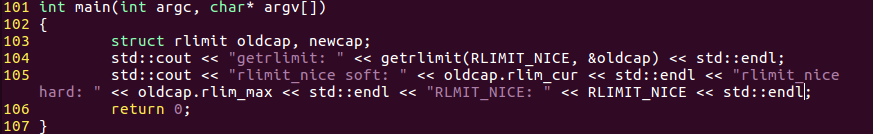
\includegraphics[width=0.9\textwidth]{../figures/systemgrundlagen/RLIMIT_NICE_code.png}}
	\subfigure[RLIMIT\_NICE output]{
		\label{RLIMIT_NICE_output}
		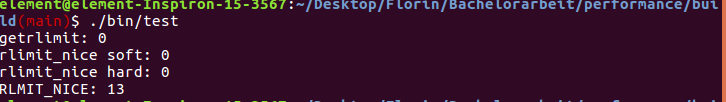
\includegraphics[width=0.9\textwidth]{../figures/systemgrundlagen/RLIMIT_NICE_output.png}}
	\caption{RLIMIT\_NICE} 
	\label{RLIMIT_NICE}
\end{figure*}
\\
Per default the process will have
the nice value of 0 and this value can be increased to the highest value allowed (19), but cannot be
decreased afterwards to a value lower than \textit{user\_nice\_value = 20-RLIMIT\_NICE}. The command \texttt{setcap} can change the executable to
run as a privileged process (but only when called as root or with the keyword sudo). A way of
increasing the nice value would be to increase the RLIMIT\_NICE value (also as root or with root-rights = sudo), which will allow a normal user to increase the value given until it reaches
\dq user\_nice\_value\dq{} or log in as root, use the library's functions, build the program and set the SUID as root.
\footnote{The SUID is a special bit that one can set and allows normal users to run the program as they
were root}\\
At last you could also modify the \dq/etc/security/limits.conf\dq{} file and set a new max nice value for a
certain user, but this is not the best solution, because that user would have the power to change
priorities not only for one program, but for all programs.
\subsubsection{Scheduling}
Unlike Windows, Linux has methods to change one's process and its threads scheduling policies.The default policy set on UNIX
is called "Round-Robin Timesharing" (SCHED\_OTHER). This allows jobs to be executed in a round robin fashion where
each process gets an equal time-slice of a CPU. There are more than one policy which can be set.
These are:
\begin{enumerate}
	\item SCHED\_OTHER
	\item SCHED\_BATCH
	\item SCHED\_IDLE
	\item SCHED\_FIFO
	\item SCHED\_RR
\end{enumerate}
The difference between SCHED\_RR and "Round Robin Timeshare"(SCHED\_OTHER) is that the realtime policy lets
us to coordinate the priorities for that schedueling policy's queue.\\
The differences are that BATCH schedules a process less
frequently, if the it gets the CPU very often and IDLE is the equivalent to a process with a nice value of 19
(very nice process <=> lowest value).
SCHED\_BATCH and SCHED\_IDLE are two normal prioritised policies, which differ from SCHED\_OTHER, but
not enough for me to focus too much on them.\\
You can get the current policy of your process by calling \texttt{int sched\_getscheduler(pid\_t pid)} from the \texttt{<sched.h>} header file. 
\\
Each of the policies mentioned above has a range of priorities levels, which can be get using the \texttt{sched\_get\_priority\_max(int policy)} and \texttt{sched\_get\_priority\_min(int policy)} methods found in \texttt{<sched.h>}.\footnote{These can be different depending on the calling xUNIX
machine}\\
On my Linux Notebook I have the following values:
\begin{figure*}[!htb]
	\centering
	\subfigure[sched\_prio\_range code]{
		\label{sched_prio_range_code}
		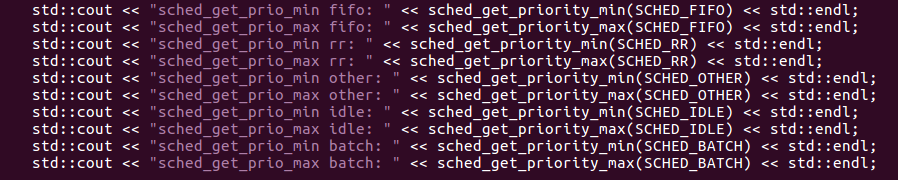
\includegraphics[width=0.9\textwidth]{../figures/sched_prio/sched_prio_range_source.png}}
	\subfigure[sched\_prio\_range output]{
		\label{sched_prio_range_output}
		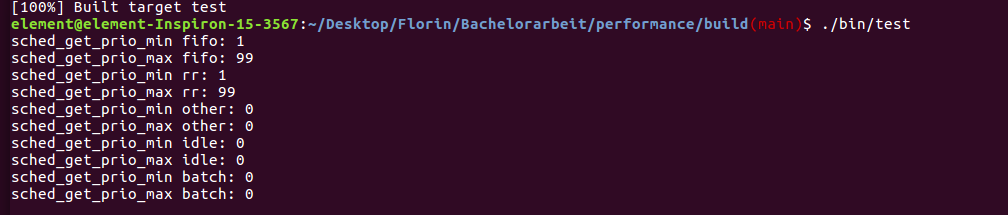
\includegraphics[width=0.9\textwidth]{../figures/sched_prio/sched_prio_range_output.png}}
	\caption{sched\_prio\_range} 
	\label{sched_prio_range}
\end{figure*}
You can only change the priority of real-time policies. hence when you set the policy of a thread to OTHER, IDLE or BATCH you can't change the priority of that process.\\
As you can observer only two of these have a \dq real\dq{} range.
SCHED\_RR and SCHED\_FIFO are characterized as real-time policies and have a higher priority than the
others. When two processes with SCHED\_RR and respectively SCHED\_FIFO have to share a CPU,
ironically the one that was placed first in that CPU's queue will get to run its job. Both of these
policies can lose access of their CPU, if they finish execution, yield\_sced() or a syscall is called
and a higher priority process preempts them (a process with a lower nice value appears in the queue
or the user changes the value himself). SCHED\_RR can also lose its access if the timeslice of
the job expires.

\section{Workload}
The definition for workload varies from field to field. In the IT-branch it is defined as a unit of measure for your CPU (mostly in \%). This tells the user how well his system can handle the number of current running processes. Most systems calculate their workload over a defined period of time. To understand this concept better, here is an example. Let's say a user starts an calculator program at time $\mathrm{t}_0$ = 0. The application will finish initializing a GUI at time $\mathrm{t}_{wait}$ = 2s and then wait for the user to enter some equation.
After the equation was typed at $\mathrm{t}_{input}$ = 5s and the "Enter"-key was pressed, the app proceeds calculating and delivering the answer at $\mathrm{t}_{done}$ = 6s. So the CPU-time of the application is 3s(GUI initialization and calculation time). In order to get its workload the system has to divide this time by the time of the system needed for the whole process $\frac{\mathrm{t}_{wait}+\mathrm{t}_{calc}}{6s}*100$.
A detailed explanation on how to get these values will follow in Chapter (*Kapitelnr*).